\documentclass{article} % Tipo de documento

\usepackage[utf8]{inputenc} % Permite el uso de caracteres del Español

\usepackage[T1]{fontenc}

\usepackage{graphicx}

\usepackage{subfig}

% Carátula del Artículo  

\title{Reporte de Actividad 8}

\author{Brenda Leyva Amaya}

\date{12 de Abril, 2018}
 

\begin{document}

\maketitle % Crea el título


\section*{Introducción}

En la presente actividad exploramos una nueva oportunidad de modelado de situaciones con jupyter lab. En esta ocasión se aborda el modelo del oscilador de Van der Pol. Con las herramientas que nos encontramos utilizando y aprendiendo a llevar a la práctica es posible observar el modelo y sus diferentes representaciones gráficas. De esta manera no solo utilizamos la herramienta matemática para la resolución de ecuaciones si no que también podemos abordar el problema de manera gráfica.

\section{Modelo de Van der Pol}

En el estudio de la dinámica, el oscilador de Van der Pol es un oscilador no conservativo con amortiguamiento no lineal. Este evoluciona o cambia con el tiempo de acuerdo a una ecuación diferencial de segundo orden. En la ecuación correspondiente x es la posición o coordenada que está en función del tiempo t y $\mu$ o en ocasiones también representada por la letra $\epsilon$ es un parámetro escalar que indica la no linealidad y la fuerza de amortiguamiento. 

\vspace{0.5 cm}

El oscilador de Van der Pol fué propuesto originalmente por el ingeniero eléctrico y físico alemán Balthasar van der Pol cuando trabajaba en Philips. Van der Pol encontró oscilaciones estables a las que posteriormente llamó oscilaciones de relajación que ahora se conocen como un tipo de ciclo límite en circuitos eléctricos que utilizan tubos de vacío. Cuando estos circuitos se llevan cerca del ciclo límite se observa un comportamiento de arrastre, esto es, que la señal directora jala o arrastra corriente con ella. Van der Pol y su colega Van der Mark, reportaron en septiembre de 1927 en un número de la revista Nature que con ciertas frecuencias se escuchó un ruido irregular que se encontró después es el resultado del comportamiento de un caos determinístico. 

\vspace{0.5 cm}

La ecuación de Van der Pol tiene un extenso historial de ser utilizada tanto en las ciencias físicas como en las biológicas. Por ejemplo en biología Fitzhugh y Nagumo extendieron la ecuación en un campo de planos como modelo para los potenciales de acción de neuronas. La ecuación también ha sido utilizada en sismología para modelar dos placas en una falla geológica y en estudios relacionados con la voz para modelar la oscilación de las cuerdas vocales.

\section{Exploración de las soluciones del modelo}

Tomando los valores iniciales X0 = 1.5 y V0 = 0.0: 

\begin{center}
	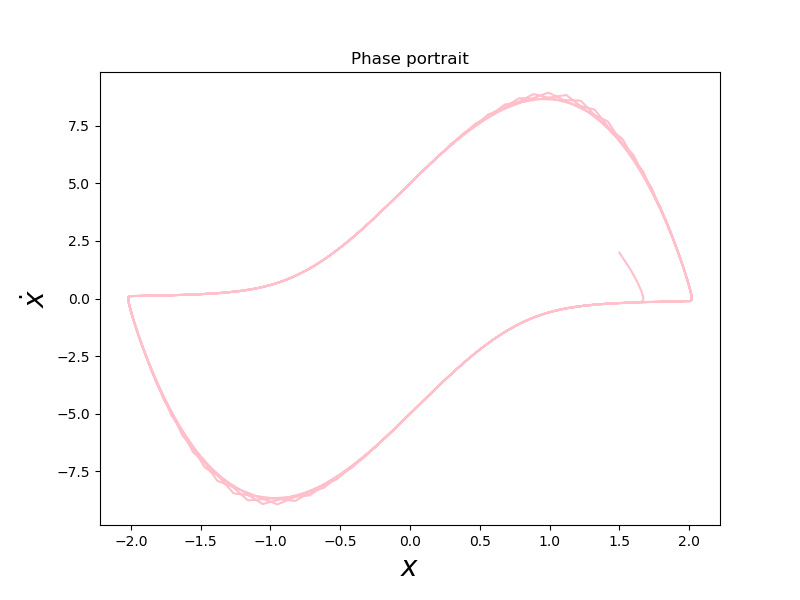
\includegraphics[width=9cm]{php1.png}
\end{center}

Tomando los valores iniciales X0 = 2.0 y V0 = 2.5: 

\begin{center}
	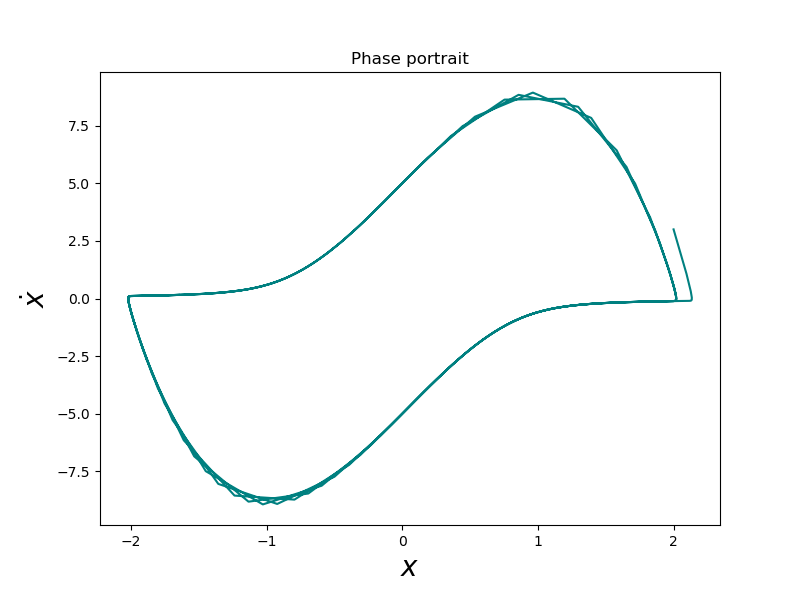
\includegraphics[width=9cm]{php2.png}
\end{center}

Tomando los valores iniciales X0 = 0.0 y V0 = 2.5: 

\begin{center}
	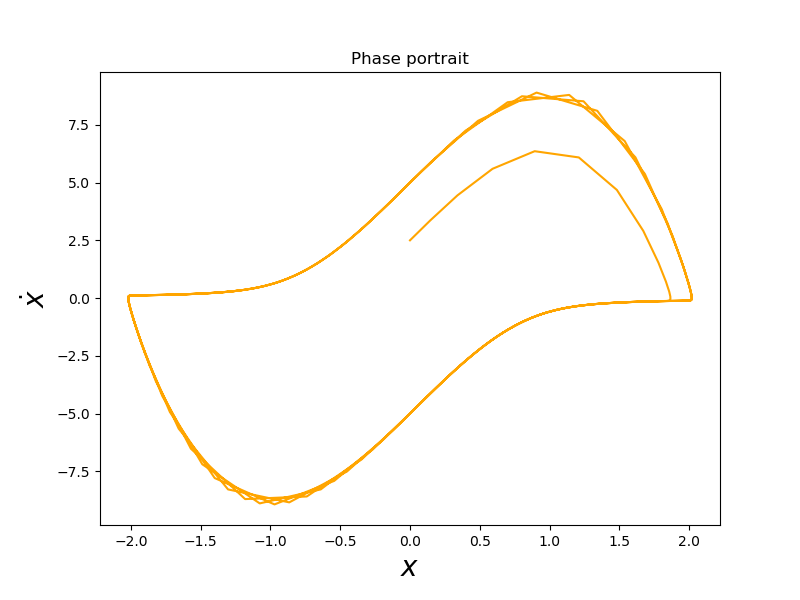
\includegraphics[width=9cm]{php3.png}
\end{center}

Tomando los valores iniciales X0 = -3.5 y V0 = 5.0: 

\begin{center}
	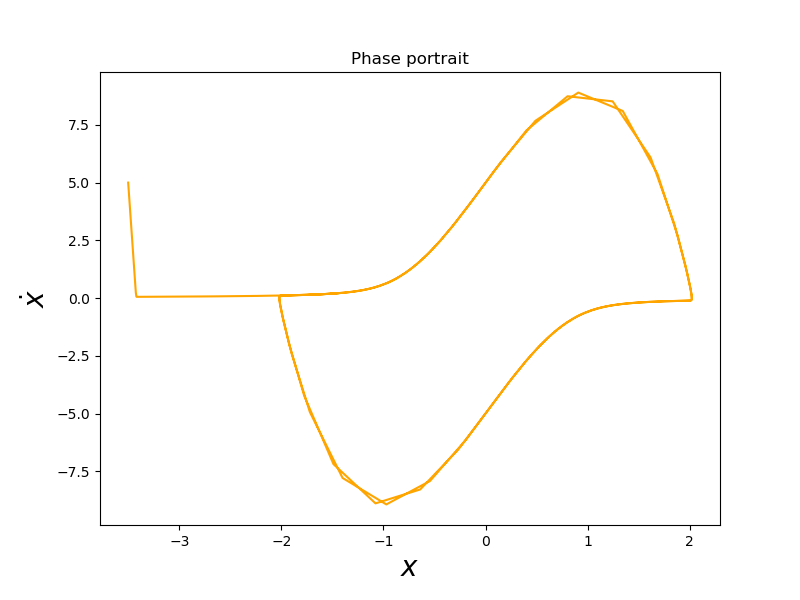
\includegraphics[width=9cm]{php4.png}
\end{center}

Es posible concluir y reflexionar que a pesar de las condiciones iniciales diferentes que se presenten, el modelo siempre reflejará el llamado ciclo límite, un punto en el cual convergen todas las soluciones y en el cual se estabilizan. 

\section{Resultados y discusión}

Finalmente se obtiene utilizando los datos propuestos por el artículo los siguientes resultados:

\vspace{0.5 cm}

**Modelado del problema. 

\begin{verbatim} 

from scipy.integrate import odeint 
from scipy import array, arange, pi, sin
import matplotlib.pyplot as plt
%matplotlib inline
from pylab import figure, plot, xlabel, grid, hold, legend, title, savefig, ylabel

def VanDerPol(X,t):
    x = X[0]
    x_point = X[1]
    dx = x_point
    dx_point = epsilon*(1 - x*x)*dx - x
    return array([dx, dx_point])

#Parámetros: 
t0 = 0
tmax = 50
pastemps = 0.05
time = arange(t0, tmax, pastemps)
x0 = 1.0
v0 = 2.0
epsilon = 2.3

x, x_point = odeint(VanDerPol,(x0,v0),time).T

with open('x4.dat', 'w') as f:
    for time, x, x_point in zip(time, x, x_point):
        print (time, x, x_point, file=f)

\end{verbatim}

**Gráfica de retrato de fase. 

\begin{verbatim} 

import numpy as np
from numpy import loadtxt
from pylab import figure, plot, xlabel, grid, hold, legend, title, savefig, ylabel
from matplotlib.font_manager import FontProperties
import matplotlib.pyplot as plt
import matplotlib.colors as colors
%matplotlib inline

p2 = plt.figure(figsize=(8,6))
t0, x, x_point = loadtxt('x1.dat', unpack=True)
figure(1, figsize=(6, 4.5))
plt.xlabel('$x$', fontsize = 20)
plt.ylabel('$\dot{x}$', fontsize = 20)
plt.plot(x, x_point, 'blue')
title('Phase portrait')

t0, x, x_point = loadtxt('x2.dat', unpack=True)
plt.plot(x, x_point, 'blue')


t0, x, x_point = loadtxt('x3.dat', unpack=True)
plt.plot(x, x_point, 'blue')


t0, x, x_point = loadtxt('x4.dat', unpack=True)
plt.plot(x, x_point, 'blue')


t0, x, x_point = loadtxt('x1.dat', unpack=True, skiprows=250)
plt.plot(x, x_point, 'red')

savefig('phportrait.png', dpi=100)

\end{verbatim}


\begin{center}
	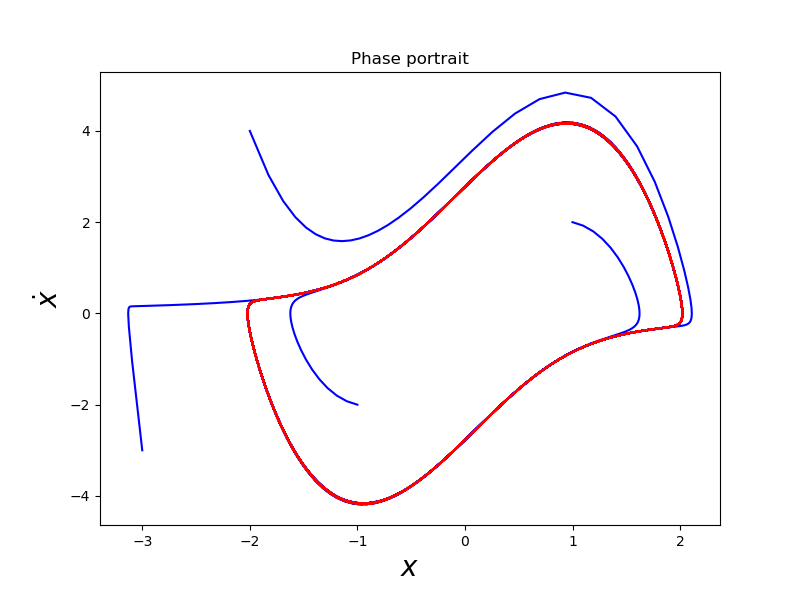
\includegraphics[width=12cm]{phportrait.png}
\end{center}

**Gráfica del ciclo límite.

\begin{verbatim} 

import numpy
from numpy import loadtxt
from pylab import figure, plot, xlabel, grid, hold, legend, title, savefig, ylabel
from matplotlib.font_manager import FontProperties
import matplotlib.pyplot as plt
%matplotlib inline

p2 = plt.figure(figsize=(4,9))
t0, x, x_point = loadtxt('e1.dat', unpack=True)
figure(1, figsize=(6, 4.5))
plt.plot(x, x_point, 'gray')
title('Evolution of the limit cycle')


t0, x, x_point = loadtxt('e2.dat', unpack=True)
plt.plot(x, x_point, 'gray')


t0, x, x_point = loadtxt('e3.dat', unpack=True)
plt.plot(x, x_point, 'gray')


t0, x, x_point = loadtxt('e4.dat', unpack=True)
plt.plot(x, x_point, 'gray')

t0, x, x_point = loadtxt('e5.dat', unpack=True)
plt.plot(x, x_point, 'gray')



t0, x, x_point = loadtxt('e6.dat', unpack=True)
plt.plot(x, x_point, 'gray')



t0, x, x_point = loadtxt('e7.dat', unpack=True)
plt.plot(x, x_point, 'gray')



t0, x, x_point = loadtxt('e8.dat', unpack=True)
plt.plot(x, x_point, 'gray')



t0, x, x_point = loadtxt('e9.dat', unpack=True)
plt.plot(x, x_point, 'gray')


t0, x, x_point = loadtxt('e10.dat', unpack=True)
plt.plot(x, x_point, 'gray')

savefig('limitcycle.png', dpi=100)

\end{verbatim}


\begin{center}
	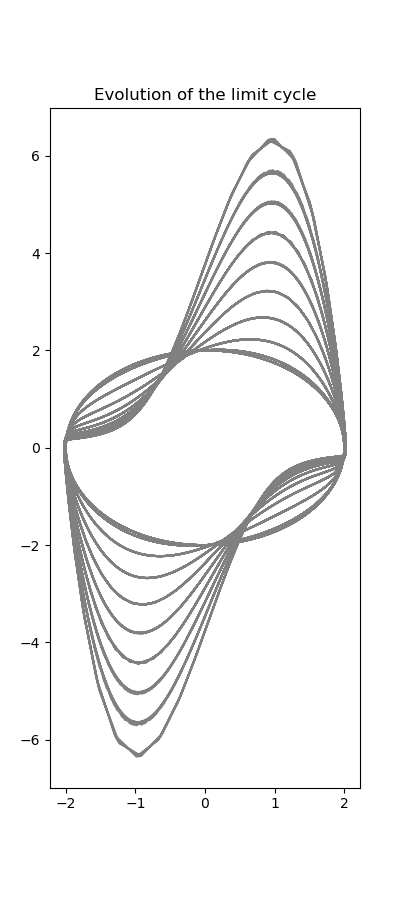
\includegraphics[width=7cm]{limitcycle.png}
\end{center}


**Gráfica de la posición en el tiempo.

\begin{verbatim} 

t0 = 10
tmax = 50
pastemps = 0.05
time = arange(t0, tmax, pastemps)

x0 = 0.0
v0 = 2.0

epsilon = 5.0

x, x_point = odeint(VanDerPol,(x0,v0),time).T
p1 = plt.figure(figsize=(10,2))
plt.grid()
plt.xlabel('$t$', fontsize = 20)
plt.ylabel('$x$', fontsize = 20)
plt.plot(time, x, 'blue')

savefig('xvst.png', dpi=100)

\end{verbatim}


\begin{center}
	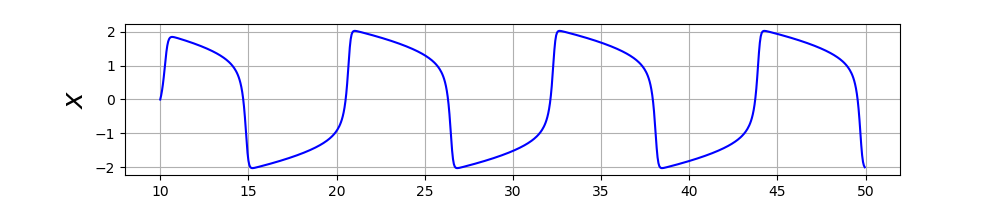
\includegraphics[width=13cm]{xvst.png}
\end{center}


**Gráfica de la posición en el tiempo.

\begin{verbatim} 

from scipy.integrate import odeint 
from scipy import array, arange, pi, sin
import numpy as np
import matplotlib.pyplot as plt
%matplotlib inline
from pylab import figure, plot, xlabel, grid, hold, legend, title, savefig, ylabel

def VanDerPol(X,t):
    x = X[0]
    a=1.2
    w=(2*np.pi)/10
    x_point = X[1]
    dx = x_point
    dx_point = epsilon*(1 - x*x)*dx - x + a*np.sin(w*t)
    return array([dx, dx_point])

#-------------------------------------------------------------------------------------

t0 = 300
tmax = 600
pastemps = 0.05
time = arange(t0, tmax, pastemps)

x0 = 0.0
v0 = 1.0

epsilon = 8.53

x, x_point = odeint(VanDerPol,(x0,v0),time).T

p1 = plt.figure(figsize=(15,3))
plt.grid()
plt.xlabel('$t$', fontsize = 20)
plt.ylabel('$x$', fontsize = 20)
plt.plot(time, x,'blue')

savefig('chaos.png', dpi=100)

\end{verbatim}


\begin{center}
	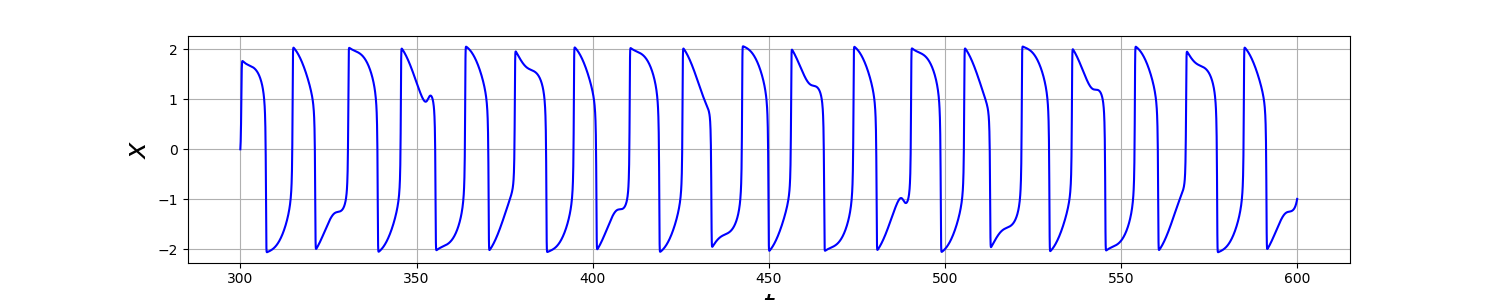
\includegraphics[width=13cm]{chaos.png}
\end{center}


\section{Conclusiones del estudio}

Al realizar esta actividad se observa la importancia o el alto impacto que tienen tanto las condiciones iniciales como el valor de la constante de no linealidad para el comportamiento final del modelo. Ha sido muy interesante observar como una modificación a estos valores se comporta gráficamente ya que elimina un un poco el sentido abstracto del modelo y lo expone en su interpretación más intuitiva. 

\section*{Bibliografía y fuentes}


\begin{verbatim} 

Van der Pol oscillator. (2018, April 10). Retrieved April 10, 2018, from
https://en.wikipedia.org/wiki/Van_der_Pol_oscillator 

\end{verbatim}


\section*{Apéndice}

\hspace{0.5 cm} Este ejercicio pareciera similar al desarrollado en las actividades 6 y 7. ¿Qué aprendiste nuevo?

\vspace{0.5 cm}

** El ejercicio se asemeja a los anteriores en las herramientas utilizadas tanto para la resolución de ecuaciones como para la graficación, sin embargo la base teórica revisada fue la de un modelo nuevo para nosotros. 

\vspace{0.5 cm}

¿Qué fue lo que más te llamó la atención del oscilador de Van der Pol?

\vspace{0.5 cm}

** Que las soluciones siempre tienden al "limit cycle".

\vspace{0.5 cm}

Has escuchado ya hablar de caos. ¿Por qué sería importante estudiar este oscilador?
 
\vspace{0.5 cm}

** Nuestra exposición al concepto de caos ha sido limitada y superficial. Es importante estudiar este tipo de modelos y comportamientos ya que son más acercados a la realidad. 

\vspace{0.5 cm}

¿Qué mejorarías en esta actividad?

\vspace{0.5 cm}

** Sería bueno complementar la actividad con una clase teórica en la cual se lleve a cabo una explicación un poco más profunda del modelo que se está revisando. 

\vspace{0.5 cm}

¿Algún comentario adicional antes de dejar de trabajar en Jupyter con Python?

\vspace{0.5 cm}

** No me siento lista para dejar de hacerlo, sería bueno obtener mayor fuidez. 

\vspace{0.5 cm}

Cerramos la parte de trabajo con Python ¿Qué te ha parecido?

\vspace{0.5 cm}

** Ha sido una experiencia muy positiva y un buen agregado a nuestro bagaje de conocimientos. 

\end{document}